
\subsection{Реализация ССМП}

\subsubsection{Использование корпуса}

%В ходе работы была попытка протестировать описанные выше подходы на 
%текстах художественной литературы. Для чистоты эксперимента,
%нужно было и обучение системы вести на художественном тексте.

В ходе работы мы попытались построить свой собственный корпус 
для обучения системы на основе <<Лолиты>> Набокова. 
Но проблема заключается в том, что такой корпус крайне сложно выровнять.
Русский и английский варианты местами сильно отличаются.
При попытке разбить на предложения наивным методом (по знакам препинания) 
расхождение возникло на $11$-м предложении.
При попытке разбить на предложения с помощью подробного 
синтаксического анализа, ошибка возникла примерно 
на $200$-м предложении.
Возможно, имеет смысл сначала разбивать текст на абзацы, 
а внутри абзацев разбивать на предложения. 
Ошибка будет иметь меньшее влияние. 
Однако сложно утверждать, 
что такой вариант не обнаружит расхождения в абзацах 
и в любом случае потребуется ручная правка и много времени.
Для маленьких корпусов существуют более сложные методы, 
такие как метод Потемкина-Кедровой \cite{Потемкин:2007}, 
но чаще всего они предполагают наличие заранее подготовленного словаря.

Обычно построение большого корпуса ведется с учетом гипотезы Гайла-Черча, о том, что 
существует прямая зависимость между длинами предложений в исходном тексте и в переводе. 
В рамках данного подхода каждой паре предложений из текстов на разных языках, 
соответствует некоторая характеристика возможности сопоставления. 
Эта характеристика вычисляется на основе разницы длин предложений 
(в символах, включая пробелы) и дисперсии этой разницы. 
Далее, с помощью методов динамического программирования, 
находится такое соответствие предложений, 
при котором характеристики возможности сопоставления максимальны \cite{Липатов:2005}.
Само по себе построение корпуса является самостоятельной задачей корпусной лингвистики.
Потому было принято решение пользоваться уже готовыми корпусами.

\pagebreak

Для  обучения рассматриваемой ССМП использовалась комбинация из нескольких русско-английских корпусов:
{\renewcommand{\labelenumi}{\alph{enumi})}
	\begin{enumerate}
		\item корпус резолюций ООН;
		\item русско-чешско-английский корпус UMC (ÚFAL Multilingual Corpora);
		\item некоторая выборка из Национального корпуса русского языка 
			(была выкачена с веб-сайта корпуса и автоматически сформирована по атрибутам тегов);
		\item некоторая выборка из работы Д. Кнута <<Искусство программирования>> 
			в качестве примера корпуса научных текстов.
	\end{enumerate}
}

Общий объем корпуса составил примерно $180`000$ 
предложений ($5`854`095$ лексических единиц) на каждом из языков.

Важно отметить, что сложно назвать полученную комбинацию корпусом научных текстов,
но за неимением хороших исходных данных пришлось довольствоваться этим.

Большие корпуса научного всего скорее у издательств, и если мы 
захотим развивать систему дальше, 
то можно будет по определенной лицензии эти корпуса приобрести.

Корпуса не обязательно будут выровнены по предложениям, 
но опираясь на свойства научного текста выравнивать 
их самостоятельно достаточно просто. 
Например это можно будет сделать, благодаря наличию формул и 
международных терминов.

\pagebreak
\subsubsection{Средство разработки}

В качестве основного инструментального средства 
используется функциональный язык erlang.

Основные преимущества:
{\renewcommand{\labelenumi}{\alph{enumi})}
	\begin{enumerate}
		\item нет побочных эффектов присущих императивным языкам;
		\item модель легковесных процессов;
		\item удобные средства разработки распределенных приложений;
		\item высокая производительность (меньше чем для~C, но~сопоставима с~C++, 
			при компиляции erlang в машинный код).
	\end{enumerate}
}
	
Очень часто erlang используют для написания высоконагруженных распределенных приложений.
Рассматриваемая система относится именно к таким приложениям.

В ходе выполнения работы как альтернативный вариант рассматривался 
язык программирования python, но после анализ данных производительности 
в рамках данной задачи предпочтение было отдано erlang.

Для увеличения надежности приложений было решено организовать 
взаимодействия процессов c учетом принципов ОТП 
(открытая телекоммуникационная платформа --- OTP, open telecom platform), 
там где это возможно. Диспетчер каждого приложения 
и модуль пула соединения с базой данных имеет 
структуру дерева контроля (<<дерева супервизии>>), как показано ниже на рисунке.
Рабочий процесс может быть обычным вычислительным сервером (в терминах OTP),
или супервизором (более низкого уровня). 
Супервизор в данном случае нужен для контроля за рабочими процессами.
Если у какого либо рабочего процесса произойдет сбой и процесс <<упадет>>, 
то супервизор перезапустит его. 

\begin{figured}
		\tikzstyle{appf} = [rectangle,thick,minimum size=1cm,draw=teal!50!black!50,top color=white,bottom color=teal!50!black!20,font=\itshape]
		\tikzstyle{supf} = [rectangle,rounded corners,thick,minimum size=1cm,draw=blue!50!black!50,top color=white,bottom color=blue!50!black!20,font=\itshape]
		\tikzstyle{wrkf} = [rounded rectangle,thick,minimum size=1cm,draw=red!50!black!50,top color=white,bottom color=red!50!black!20,font=\itshape]
	\begin{tikzpicture}[thick, node distance=4cm, text height=1.5ex, text depth=.25ex, auto]
		\node[appf] 			(app)	{Приложение (в терминах ОТП)};
		\begin{scope}[node distance=2cm]
			\node[supf,below of=app]	(sup)	{Супервизор};
		\end{scope}		
		\begin{scope}[node distance=3.5cm]
			\node[wrkf,below left of=sup]	(wrk1)	{Рабочий процесс $1$};
			\node[wrkf,below right of=sup]	(wrkn)	{Рабочий процесс $n$};
		\end{scope}		
		\node[wrkf,below of=sup]		(wrkd)	{Рабочий процесс $\ldots$};
			
		\path[<->, blue] 				(app)	edge (sup);
		\path[<->, red] 				(sup)	edge (wrk1);
		\path[<->, red] 				(sup)	edge (wrkd);
		\path[<->, red] 				(sup)	edge (wrkn);
	\end{tikzpicture}
	\fcaption{Дерево контроля ОТП.}
\end{figured}

Если сбои будут происходит 
в течение заранее определенного промежутка времени то супервизор 
передаст сигнал о том, что про процесс перестал работать вверх 
по дереву контроля.

Если приложение (в терминах ОТП) контролируется другим супервизором, то процесс повторится снова.
И так пока не дойдет до самого верхнего уровня, что приведет к отказу самого приложения.

\subsubsection{База данных}

В качестве базы данных используется Redis Server.
Ранее были рассмотрены прочие варианты:
\begin{enumerate}
	\item Хранить все словари в памяти, а по окночании скидывать на диск --- очень 
		быстро, но опасно, ибо когда память кончится программа начинает работать не стабильно.
	\item Использовать локальное отображение в файл --- но такой вариант:
	\begin{itemize}
		\item очень медленный;
		\item не масштабируемый.
	\end{itemize}
	\item Попробовали в качестве базы данных использовать Memcache, но оно оказалось 
	медленно, и нет поддержки атомарных операций.
	\item Попробовали в качестве базы данных использовать родные для erlang dts и mnesia, 
		но первая имеет ограничение в размере хранимых данных,
		вторая в количестве хранимых ключей.
\end{enumerate}
В результате долгих поисков и анализа, мы пришли к текущему варианту
Кроме того, Redis версии ниже 2.4 оказался чувствителен к длине ключей и значений. 

Важной особенностью Redis является поддержка атомарных операций обновления,
работа с множествами и списками, работа с хранилищами типа ключ-значение.
Для реализации алгоритмической части были крайне необходимы следующие операции:
\begin{ditemize}
	\item  для работы с $n$-грамами:
	\begin{itemize}
		\item {\tt sadd key value } --- добавить элемент в множество,
		\item {\tt srandmember key  } --- получить случайный элемент множества,
		\item {\tt smove source destination member } --- переместить элемент из одного множества в другое;
	\end{itemize}
	\item для работы со списками $n$-грам:	
	\begin{itemize}
		\item {\tt lpush key value } --- добавление элемента в начало списка,
		\item {\tt rpush key value } --- добавление элемента в конец списка,
		\item {\tt lpop key } --- получение первого элемента списка и его удаление,
		\item {\tt rpop key } --- получение последнего элемента и его удаление,
		\item {\tt rpoplpush srckey dstkey} --- получение и удаление последнего 
			элемента списка {\tt <<srckey>>} с добавлением его в {\tt <<dstkey>>};
	\end{itemize}
	\pagebreak
	\item  для работы с подсчетами и оценкой вероятности:
	\begin{itemize}
		\item {\tt hset key field value } --- установить значение поля,
		\item {\tt hget key field} --- получить значение поля,
		\item {\tt hincrby key field integer} --- увеличить значение поля {\tt <<field>>}
			на~заданную величину {\tt <<integer>>},
		\item {\tt hexists key field } --- проверить существование поля.
	\end{itemize}
\end{ditemize}
Все эти операции имеют константное время доступа.

Учитывая характер системы, достаточно узким ее местом
является скорость доступа к базе данных, особенно, если база является удаленной.
Наличие асинхронных операций записи при вычисления подсчетов в данном 
случае является огромным преимуществом, 
Мы используем параллельный доступ к базе данных. 
Это особенно оказывается критично на синхронных 
операциях чтения.

Для параллельного доступа к базе данных, и исключения блокировок 
мы используем пул соединений с базой данных.
Ниже на рисунке представлено дерево контроля потоков пула соединения. 

\begin{figured}
	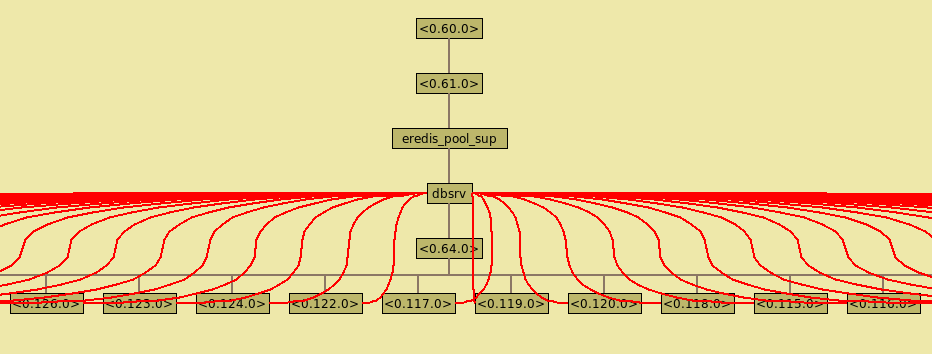
\includegraphics[width=16cm]{./img/practice-dbpool.png}
	\caption{Дерево контроля для пула соединения.}
\end{figured}

\pagebreak

\subsubsection{Арифметика с фиксированной запятой}

В результате деления при осуществлении сбора подсчетов используется вещественное деление.
Для инкремента подсчетов удобно использовать атомарную операцию {\tt hincrby}.
Однако, она работает только с целыми числами. В этом случае мы предлагаем следующий подход.

В качестве вероятности, мы будем использовать числа с фиксированной запятой
по основанию $576460752303423488$ ($2^{59}$). Такое число выбрано не~случайно,
это максимальное положительное число используемое в erlang,
которое может поместиться в машинное слово 64-битной архитектуре.
\[
	Base := 576460752303423488;
\]
%	adiv(X, Y, Base)->   round(Base / Y * X).
\[
	\mathrm{adiv}(X, Y)	\rightarrow \left\lfloor \dfrac{Base}{Y} \cdot X \right\rfloor.
\]
%	amul(X, Y, Base)->   round(X / Base * Y).
\[
	\mathrm{amul}(X, Y)	\rightarrow \left\lfloor \dfrac{X}{Base } \cdot Y \right\rfloor.
\]

При таком подходе возможно появления ошибок гораздо большего порядка, 
чем существующее машинное <<эпсилон>>, но они все равно будут пренебрежимо малы.
Для скорости вычислений и экономии памяти, важно соблюсти
последовательность вычислений.

По проведенном тестам прирост скорости составил примерно 14~раз при~применении 
операции {\tt hincrby} c~числами с~фиксированной запятой, по~сравнению с~последовательными
считывании и~записью в~базу данных.

\subsubsection{Обучение системы}

Основой системы являются базовые алгоритмы моделей IBM 1 и IBM 2 
(можно найти в приложении).
Причем с точки зрения эффективности автор отдает предпочтении IBM 1.
При использовании IBM 2 при падении производительности 
улучшения качества работы системы не замечено было.

В большинстве случаев 
для полной сходимости было достаточно около $10$ итераций. 
Потому в рабочей системе предлагается условие сходимости заменить 
проверкой значения счетчика цикла. 

\paragraph{Инициализация}

В базовом алгоритме указано, что необходимо перед началом его работы 
инициализировать величины $t(\WE|\WR)$ для всех $\WE$ и $\WR$ 
в параллельном корпусе. Логично было бы для этого использовать абсолютную
частоту слова в каждом подкорпусе. Однако, для этого необходимо 
прочитать весь корпус целиком. Если внимательно посмотреть на базовый 
алгоритм, то становится ясно, что от начального значения величин
$t(\WE|\WR)$ ничего не зависит, если они все одинаковы.
В таком случае, можно их инициализировать 
заранее какой-либо константой, например 
в данной работе используется константа равная $0.5$.
 
\paragraph{Возможные ошибки}

Очень важным моментом реализации алгоритма обучения является то,
что оценка вероятности модели и вычисления подсчетов должны происходить
сразу по всему корпусу текстов.

На начальных этапах реализации системы нами была допущено серьезная ошибка.
Приложения читателя, проходила по корпусу и считывало 1000 строк.
После этого эта тысяча строк отправлялась на обработки и по ней строилась модель
перевода. Затем считывалась следующая порция строк.

В результате этих действий подсчеты вычислялись только для локального набора строк,
и затем по ним вычислялась вероятность переводных соответствий и перезаписывала 
вероятность вычисленную ранее.

После окончания работы алгоритма обучения мы получали вероятности 
переводных соответствий обученные только на последней тысяче строк, 
с некоторым влиянием остального корпуса.

Установить ошибку удалось только после запуска алгоритма в предельном случае
на корпусе состоящим из двух строк, при проходе полного алгоритма
обучения на каждой из них.

\pagebreak
\subsubsection{Реализация интерфейсов декодера}

Рассматриваемая система обладает тремя видами интерфейса:
\begin{itemize}
	\item консольные;
	\item простой веб-интерфейс;
	\item rest-интерфейс.
\end{itemize}

Консольное приложение является стандартным отладочным интерфейсом ОТП приложений.
Для перевода достаточно просто  вызывать соответствующую функцию модуля.

Веб-интерфейс декодера выполнен в виде отдельного ОТП приложения и представляет
из себя полноценный веб-ресурс, реализованный с помощью библиотеки mochiweb.

Мы не будем в работе приводить как внешне выглядит клиентская часть Веб-приложения,
которая отображается в браузере, так как она представляет собой всего лишь текстовый элемент ввода,
две кнопки (<<перевести>> и <<улучшить перевод>>), и текстовый элемент вывода.

Важнейшей частью Веб-приложения является XSLT-преобразователь.
В данном случае он был написан на С c использованием libxml2 и libxslt.
Из erlang он вызывается как порт-сервер. На вход подается строка XML 
которая содержит в себе данные (в нашем случае, это перевод исходного текста в случае ответа на запрос)
и шаблон XSL, в котором описано как данные передавать.
Для увеличения быстродействия XSLT преобразователь (на стороне кода на C) 
использует хэш-таблицу, в которой записываются использованные ранее XSL шаблоны. 
Сделано для того, чтобы не загружать при повтором обращении каждый шаблон снова.
В рамках проекта было реализовано две версии преобразователя c запоминанием шаблонов и без него.
Версия без хэш-таблицы работает медленнее, но удобнее при <<горячей замене>> шаблона 
уже на работающем коде.
Кроме того, преобразователь является не блокирующим и при одновременных обращениях
вызывается параллельно. Последнее дает прирост производительности 
при наличие нескольких процессоров или ядер.

Rest-интерфейс декодера также выполнен в виде отдельного ОТП приложения и представляет
из себя полноценный веб-ресурс реализованный с~помощью библиотеки mochiweb.

После поступления POST запроса приложению, оно начинает 
передавать текстовый (Content-Type: text/plain) 
HTTP (chunked) поток с~наиболее вероятными вариантами перевода. 
Этот поток будет передаваться до тех пор, 
пока клиент не закроет соединение, 
или не будут перебраны все варианты улучшения перевода.

Поток представляет из себя набор чанков в рамках спецификации протокола HTTP 1.1.
Каждый чанк содержит количество передаваемых байт и последовательность передаваемых данных.

Каждая строка полного перевода исходного текста передается 
в отдельном чанке и обязательно заканчивается 
символом перевода строки.

В отличие от web-интерфейса в этом случае клиенту не нужно будет самому
запрашивать улучшение перевода. Самый первый <<жадный>> вариант перевода 
передается в первом чанке потока.

\pagebreak

